\documentclass[10pt,a4paper]{article}
\usepackage[utf8]{inputenc}
\usepackage[T1]{fontenc}
\usepackage{amsmath}
\usepackage{amsfonts}
\usepackage{amssymb}
\usepackage{graphicx}
\usepackage{tikz}
\usepackage{float}
\usepackage{tikz-cd}


\usetikzlibrary{calc,arrows.meta,positioning}

\tikzset{
	every node/.style={font=\sffamily\small},
	main node/.style={thick,circle,draw,font=\sffamily\Large}
}

\usepackage[backend = biber, style=authoryear]{biblatex}
\addbibresource{bibliography.bib}

\usetikzlibrary{fit,positioning}

\author{Gabriel Wallin}
\title{Some notes on state-space LBM}

\begin{document}
\maketitle

\section{The Extended SIR model}
To specify the State-Space Latent Block Model (SS-LBM), we introduce the following notation: 
%
$
\mathbf{y} = (\mathbf{y}_{it}, i = 1, \ldots, n; t = 1, \ldots T) 
$
%
denotes the data matrix which is a multivariate time series:  
%
$
\mathbf{y}_{it} = (y_{i}^1(t), \ldots, y_{i}^S(t))
$ 
%
where $t \in [0, T]$. In the context of analyzing the 2020 coronavirus pandemic, 
%
$
\mathbf{y}_{it} = (y_{i}^I(t), y_{i}^R(t))^\top
$
%
where $y_{i}^I(t)$ and $y_{i}^R(t)$ denote the proportion of infected and removed (recovered or dead) by the virus, respectively, at time point $t$. Further, let  
%
$
\boldsymbol{\theta} = (\theta_t^S, \theta_t^I, \theta_t^R)^\top,
$
%
where $\theta_t^S$, $\theta_t^I$ and $\theta_t^R$ is the probability of a person being susceptible, infected and removed, respectively, at time point $t$. We will assume that 
%
$
\boldsymbol{\theta}_{0:T} = (\boldsymbol{\theta}_0, \boldsymbol{\theta}_1, \ldots, \boldsymbol{\theta}_T)
$
%
is a first-order Markov chain in the same spirit as \parencite{osthus2017forecasting} and \parencite{song2020epidemiological}. This implies that 
%
$
g(\boldsymbol{\theta}_t|\boldsymbol{\theta}_{0:(t-1)}) = g(\boldsymbol{\theta}_t|\boldsymbol{\theta}_{t-1}) \, \forall t \in [0:T]. 
$
%
Specifically, we assume the following model for $\boldsymbol{\theta}$:
%
$$
\boldsymbol{\theta}_t | \boldsymbol{\theta}_{t-1}, \boldsymbol{\Omega}_1 \sim \text{Dirichlet}(\kappa f(\theta_{t-1}^S), \kappa f(\theta_{t-1}^I), \kappa f(\theta_{t-1}^R)),
$$
where $\boldsymbol{\Omega}_1$ denotes the set of model parameters, $\kappa$ scales the variance of the Dirichlet distribution, and the function $f(\cdot)$ is a 3-dimensional vector that sets the mean of the Dirichlet distribution.
%

The function $f$ is the solution to the following dynamic system:
%
\begin{equation}\label{SIR}
	\frac{d\theta_t^S}{dt} = -\rho\pi(t)\theta_t^S\theta_t^I, \quad \frac{d\theta_t^I}{dt} = \rho\pi(t)\theta_t^S\theta_t^I - \gamma \theta_t^I, \quad \frac{d\theta_t^R}{dt} = \gamma \theta_t^I,
\end{equation}
%
where $\rho > 0$ is the transmission rate of the disease, and $\gamma > 0$ is the rate of recovery. The term $\pi(t)$ is a transmission modifier equal to $\pi(t) = (1-q^S(t))(1-q^I(t))$, where $q^S(t)$ denotes the probability of an susceptible person being in-home isolation, and $q^I(t)$ the probability of an infected person being in-hospital quarantine. The term $\pi(t)$ is a transmission modifier in the sense that it modifies the probability of a susceptible person getting in contact with an infected person. If a geographical region does not impose a quarantine, $\pi(t)=1$, and the dynamic system in \ref{SIR} reduces to the clasic formulation of the SIR model \parencite{kermack1927contribution}. We are however considering the extended version, for which the $\pi(t)$ term is included. Since there are no explicit solutions available to (\ref{SIR}), the so-called fourth-order Runge-Kutta approximation is implemented, meaning that 
%
$$
\begin{aligned}
	\begin{pmatrix}
		f(\theta_{t-1}^S) \\
		f(\theta_{t-1}^I) \\
		f(\theta_{t-1}^R)
	\end{pmatrix}
\end{aligned} = 
%
\begin{aligned}
	\begin{pmatrix}
		\theta_{t-1}^S + 1/6[k_{t-1}^{\theta^S_1} + 2k_{t-1}^{\theta^S_2} + 2k_{t-1}^{\theta^S_3} + k_{t-1}^{\theta^S_4}] \\
		\theta_{t-1}^I + 1/6[k_{t-1}^{\theta^I_1} + 2k_{t-1}^{\theta^I_2} + 2k_{t-1}^{\theta^I_3} + k_{t-1}^{\theta^I_4}] \\
		\theta_{t-1}^R + 1/6[k_{t-1}^{\theta^R_1} + 2k_{t-1}^{\theta^R_2} + 2k_{t-1}^{\theta^R_3} + k_{t-1}^{\theta^R_4}]
	\end{pmatrix}
\end{aligned}
$$
%
where 
%
\begin{equation*}
\begin{split}	
		k_{t-1}^{\theta^S_1} &= - \rho \theta_{t-1}^S \theta_{t-1}^I, \\
		%
		k_{t-1}^{\theta^S_2} &= - \rho [\theta_{t-1}^S + 0.5 k_{t-1}^{\theta^S_1}] [\theta_{t-1}^I + 0.5 k_{t-1}^{\theta^I_1}], \\
		%
		k_{t-1}^{\theta^S_3} &= \rho [\theta_{t-1}^S + 0.5 k_{t-1}^{\theta^S_2}] [\theta_{t-1}^I + 0.5 k_{t-1}^{\theta^I_2}], \\
		%
		k_{t-1}^{\theta^S_4} &= \rho [\theta_{t-1}^S + k_{t-1}^{\theta^S_3}] [\theta_{t-1}^I + k_{t-1}^{\theta^I_3}],
\end{split}
\end{equation*}
%
\begin{equation*}
	\begin{split}	
		k_{t-1}^{\theta^I_1} &= \rho \theta_{t-1}^S \theta_{t-1}^I - \gamma \theta^I_{t-1}, \\
		%
		k_{t-1}^{\theta^I_2} &= \rho [\theta_{t-1}^S + 0.5 k_{t-1}^{\theta^S_1}] [\theta_{t-1}^I + 0.5 k_{t-1}^{\theta^I_1}] - \gamma[\theta_{t-1}^I + 0.5 k_{t-1}^{\theta^I_1}], \\
		%
		k_{t-1}^{\theta^I_3} &= \rho [\theta_{t-1}^S + 0.5 k_{t-1}^{\theta^S_2}] [\theta_{t-1}^I + 0.5 k_{t-1}^{\theta^I_2}] - \gamma[\theta_{t-1}^I + 0.5 k_{t-1}^{\theta^I_2}], \\
		%
		k_{t-1}^{\theta^I_4} &= \rho [\theta_{t-1}^S + k_{t-1}^{\theta^S_3}] [\theta_{t-1}^I + k_{t-1}^{\theta^I_3}] - \pi[\theta_{t-1}^I + k_{t-1}^{\theta^I_3}], 
	\end{split}
\end{equation*}
%
and 
%
\begin{equation*}
	\begin{split}	
		k_{t-1}^{\theta^R_1} &= \gamma \theta^I_{t-1}, \\
		%
		k_{t-1}^{\theta^R_2} &= \gamma[\theta_{t-1}^I + 0.5 k_{t-1}^{\theta^I_1}], \\
		%
		k_{t-1}^{\theta^R_3} &= \gamma[\theta_{t-1}^I + 0.5 k_{t-1}^{\theta^I_2}], \\
		%
		k_{t-1}^{\theta^R_4} &= \gamma[\theta_{t-1}^I + k_{t-1}^{\theta^I_3}]. 
	\end{split}
\end{equation*}
%

Lastly, for the data $\mathbf{y}$  we follow \parencite{song2020epidemiological} and make the following distributional assumptions,  
%
\begin{equation}\label{statespace}
\begin{aligned}
	y_{i}^I(t) | \boldsymbol{\theta}, \boldsymbol{\Omega}_1 \sim \text{Beta}(\lambda^I \theta_t^I, \lambda^I(1 - \theta_t^I)) \\
	%
	y_{i}^R(t) | \boldsymbol{\theta}, \boldsymbol{\Omega}_1 \sim \text{Beta}(\lambda^R \theta_t^R, \lambda^R(1 - \theta_t^R)
\end{aligned}
\end{equation}
%
where 
%
$
\boldsymbol{\Omega}_1 = (\rho, \gamma, \mathbf{\theta}, \lambda, \kappa)^\top.
$
%
We consequently have a state-space formulation of the considered model, where $\boldsymbol{\theta}$ is the underlying, latent process that guides the observed data $(y_i^I(t), y_i^R(t))$. This state-space extended SIR model can be graphically summarized as


\begin{figure}[H]
	\centering
	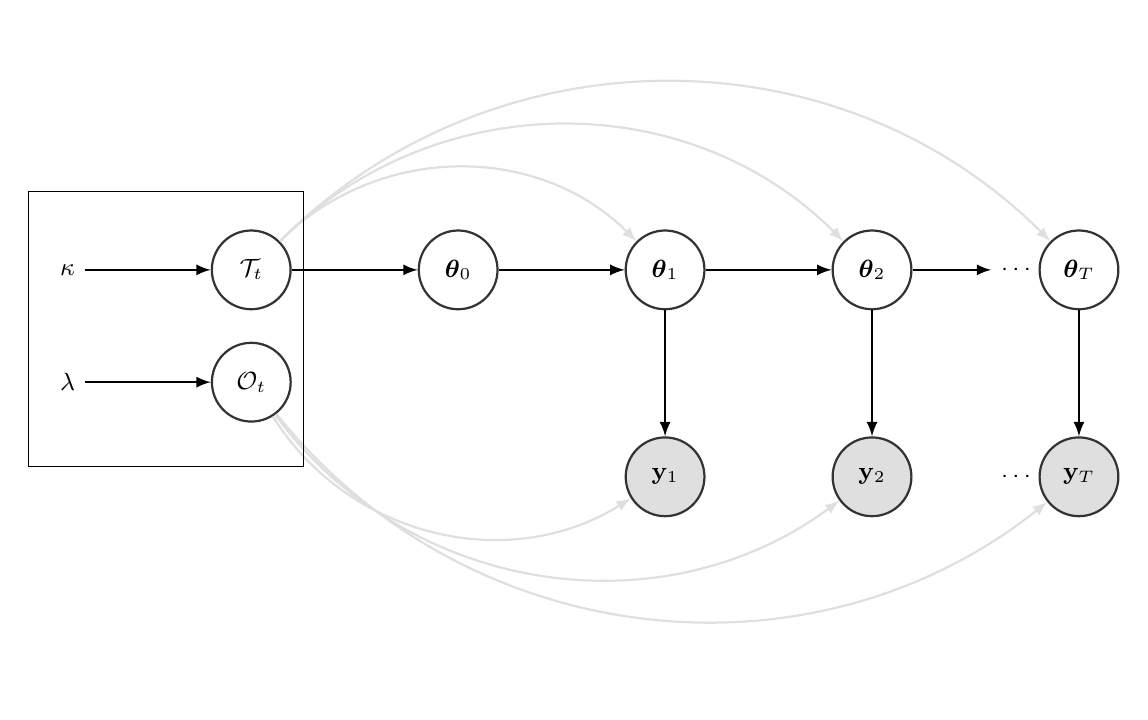
\begin{tikzpicture}
		\tikzstyle{main}=[circle, minimum size = 10mm, thick, draw =black!80, node distance = 16mm]
		\tikzstyle{connect}=[-latex, thick]
		%\tikzstyle{box}=[rectangle, draw=black!100]
		\node[ fill = white!100] (kappa) {$\kappa$};
		\node[main] (T) [right=of kappa] {$\mathcal{T}_t$};
		
		\node[] (lambda) [below=of kappa] {$\lambda$};
		\node[main] (O) [right=of lambda] {$\mathcal{O}_t$};
		
		\node[main] (theta0) [right=of T] {$\boldsymbol{\theta}_0$};
		\node[main] (theta1) [right=of theta0] {$\boldsymbol{\theta}_1$};
		\node[main] (theta2) [right=of theta1] {$\boldsymbol{\theta}_2$};
		\node[main] (thetaT) [right=of theta2] {$\boldsymbol{\theta}_T$};
		
		\node[main, fill = gray!25] (y1) [below=of theta1] {$\mathbf{y}_1$};
		\node[main, fill = gray!25] (y2) [right=of y1] {$\mathbf{y}_2$};
		\node[main, fill = gray!25] (yT) [right=of y2] {$\mathbf{y}_T$};
		
		
		\path (kappa) edge [connect] (T);
		\path (lambda) edge [connect] (O);
			
		\path (T) edge [connect] (theta0);
		
		\path (theta0) edge [connect] (theta1);
		\path (theta1) edge [connect] (theta2);
		
		\path (theta1) edge [connect] (y1);
		\path (theta2) edge [connect] (y2);
		\path (thetaT) edge [connect] (yT);
		
		\node[] (dots) [right=of theta2]{\ldots};
		\node[] (dotsy) [right=of y2]{\ldots};
		
		\path (theta2) edge [connect] (dots);
		
		\path[bend right=45, color = gray!25] (O) edge [connect] (y1);
		\path[bend right=45, color = gray!25] (O) edge [connect] (y2);
		\path[bend right=45, color = gray!25] (O) edge [connect] (yT);
	
    	\path[bend left=45, color = gray!25] (T) edge [connect] (theta1);
	    \path[bend left=45, color = gray!25] (T) edge [connect] (theta2);
		\path[bend left=45, color = gray!25] (T) edge [connect] (thetaT);
		
		\draw[] (-0.5,-2.5) rectangle (3,1);
	
	\end{tikzpicture}
\end{figure}	



%\begin{tikzcd}[nodes in empty cells]
%	\text{Markov process:}
%	&   \boldsymbol{\theta}_0
%	&   \boldsymbol{\theta}_1 \ar[dd]
%	&   \boldsymbol{\theta}_2  \ar[dd]
%	&   \dots  
%	&   \boldsymbol{\theta}_{T-1} \ar[dd]       \\
%	&   \arrow[rrrr, dashed, -,
%	start anchor={[shift={(-3ex,2ex)}]north west},
%	end anchor  ={[shift={( 3ex,2ex)}]north east}]
%	&   &   &   &   &                               \\
%	\text{Observations:}
%	&   \mathbf{y}_0
%	&   \mathbf{y}_1
%	&   \mathbf{y}_2
%	&   \dotsm
%	&   \mathbf{y}_{T-1}           \\
%\end{tikzcd}

Returning back to the analysis of the 2020 coronavirus epidemic, with $n$ countries measured on $T$ time points, the data matrix $\mathbf{y}$ that we wish to co-cluster thus equals
%
$$
\mathbf{y} = \begin{bmatrix}
	(y^I_1(1), y^R_1(1)) & (y^I_1(2), y^R_1(2)) & \ldots & (y^I_1(T), y^R_1(T))\\
	(y^I_2(1), y^R_2(1)) & (y^I_2(2), y^R_2(2)) & \ldots & (y^I_2(T), y^R_2(T))\\
	\vdots & \vdots & \ldots & \vdots \\
	(y^I_n(1), y^R_n(1)) & (y^I_n(2), y^R_n(2)) & \ldots & (y^I_n(T), y^R_n(T))
\end{bmatrix}
$$
%

\section{Latent Block Model}
Following the latent block model (LBM; \cite{govaert2003clustering}), we assume that there is a partition ($Z$, $W$) of the data matrix $\mathbf{y}$, for which $Z$ is partitioned into $K$ clusters on the $n$ rows and $W$ is partitioned into $L$ clusters on the $T$ columns. In other words, $Z_{ik}$, $k = 1,..., K$ and $W_{tl}$, $l = 1,..., L$ are binary matrices for which $Z_{ik} = 1$ if case $i$ belongs to row cluster $k$ and $0$ otherwise, and $W_{jl} = 1$ if time point $t$ belongs to column cluster $l$ and $0$ otherwise. The random matrices $Z$ and $W$ therefore are of dimension $n \times K$ and $T \times L$, respectively. 

Co-clustering will yield subgroups, called blocks, such that $Z_{ik} W_{tl} = 1$. Each element $\mathbf{y}_{it}$ in $\mathbf{y}$ belongs to a block which is generated by a probability distribution. In this study it is assumed that $y_{i}^I(t)$ and $y_{i}^R(t)$ follow Beta distributions, meaning that these block distributions are given by the distributions specified by Equation \ref{statespace}. It is assumed that $Z$ and $W$ are independent from each other and that the random variables $\mathbf{y}$ are independent conditional on $Z$ and $W$.

Now let $\alpha_k = P(Z_{ik} = 1)$ and $\beta_l = P(W_{jl} = 1)$ denote the respective row and column mixing proportions such that they both sum to 1 and 
%
$
p(z; \theta) = \prod_{ik} \alpha_k^{z_{ik}} 
$
%
and 
%
$
p(w; \theta) = \prod_{ik} \beta_l^{w_{jl}}. 
$ 
%
Under the assumption of $Z$ and $W$ being independent, and by letting $\mathcal{Z}$ and $\mathcal{W}$ denote the sets of all possible partitions of $Z$ and $W$, the likelihood of the LBM equals
$$
L(\boldsymbol{\Omega}_2) = \sum_{(z, w) \in \mathcal{Z}, \mathcal{W}} \prod_{i, g} \alpha^{z_{ig}} \prod_{j, l} \beta^{w_{jl}} \prod_{i, j, k, l} \varphi(\mathbf{y}_{ij}; \omega_{kl})^{z_{ig} w_{jl}},
$$
%
where $\omega_{kl}$ represents the parameter of $\varphi$ for the $kl$ block. The log-likelihood equals 
%
$$
\log L(\boldsymbol{\Omega}_2) = \sum_{i, k} z_{ik} \log\alpha_k \sum_{j, l} w_{jl} \log \beta_l \sum_{i, j, k, l} z_{ik} w_{jl} \log\varphi(\mathbf{y}_{ij}; \omega_{kl}),
$$
%

The state-space LBM can now graphically be represented as

\begin{figure}[H]
	\centering
	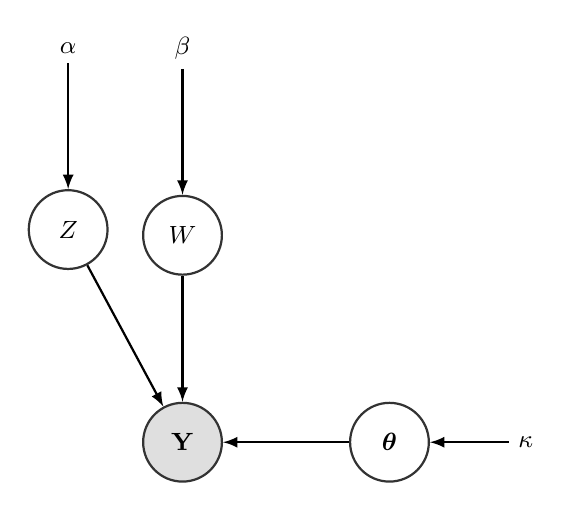
\begin{tikzpicture}
		\tikzstyle{main}=[circle, minimum size = 10mm, thick, draw =black!80, node distance = 16mm]
		\tikzstyle{connect}=[-latex, thick]
		%\tikzstyle{box}=[rectangle, draw=black!100]
		\node[ fill = white!100] (alpha) {$\alpha$};
		\node[main] (Z) [below=of alpha] {$Z$};
		
		\node[] (beta) [right=of alpha] {$\beta$};
		\node[main] (W) [below=of beta] {$W$};
		
		\node[main, fill = gray!25] (Y) [below=of W] {$\mathbf{Y}$};
		\node[main] (theta) [right=of Y] {$\boldsymbol{\theta}$};
		
		\node[] (kappa) [right=of theta] {$\kappa$};
		
		\path (Z) edge [connect] (Y);
		\path (W) edge [connect] (Y);
		
		\path (theta) edge [connect] (Y);
		
		\path (alpha) edge [connect] (Z);
		\path (beta) edge [connect] (W);
		
		\path (kappa) edge [connect] (theta);
		
		%\node[rectangle, inner sep=0mm, fit= (z) (w),label=below right:N, xshift=13mm] {};
		%\node[rectangle, inner sep=4.4mm,draw=black!100, fit= (z) (w)] {};
		%\node[rectangle, inner sep=4.6mm, fit= (z) (w),label=below right:M, xshift=12.5mm] {};
		%\node[rectangle, inner sep=9mm, draw=black!100, fit = (theta) (z) (w)] {};
	\end{tikzpicture}
\end{figure}	


\section{Estimation}

Since there are two model components of the eSIR LBM, we repeat the total set of parameters that needs to be estimated. The unknown parameters from the eSIR model component of the likelihood thus equals 
%
$ 
\boldsymbol{\Omega}_1 = (\rho, \gamma, \boldsymbol{\theta}, \lambda, \kappa)
$ 
%
and the LBM model component of the likelihood equals
%
$ 
\boldsymbol{\Omega}_2 = (\alpha, \beta, \omega).
$ 
%
The total set of parameters to be estimated thus equals 
%
$
\boldsymbol{\Omega} = \boldsymbol{\Omega}_1 + \boldsymbol{\Omega}_2 = (\rho, \gamma, \boldsymbol{\theta}, \lambda, \kappa, \alpha, \beta, \omega).
$
%

For the estimation of the eSIR LBM model, we will assume that $\varphi(\mathbf{y}_{ij}; \omega_{kl})$ follows a Dirichlet distribution:
%
$$
\varphi(\mathbf{y}_{ij}; \omega_{kl}) = D(\omega_{kl})^{-1} \prod_{j=1}^{d+1} y_{ij}^{\omega_{kl}-1}
$$
%
So should we model $\varphi(\cdot)$ as a bivariate beta distribution (meaning Dirichlet distribution)? Regarding this, see the paper "Time Series of Continuous Proportions", by Grunwald, Raftery and Guttorp (1993), where they model the time series of proportions using the Dirichlet distribution.


There is a paper ("Estimation and selection for the latent block model on categorical data" by Keribin et al.) that implements the LBM for multinomial data that in the estimation of the model sets prior distributions for the mixing proportions as well as the parameter that governs the $Y$ distribution. This would in a sense be similar to our case, since the eSIR model imposes a Dirichlet prior on the $\boldsymbol{\theta}$ parameter. If we would further impose Dirichlet priors on the mixing proportions, would we be able to do something similar as in Keribin et al.?

So specifically, following \parencite{keribin2015estimation} we can consider proper and non-informative priors for $\alpha$ and $\beta$ as
%
\begin{equation}
	\begin{aligned}
		\boldsymbol{\alpha} \sim \text{Dirichlet}(a, \ldots, a) \\
		%
		\boldsymbol{\beta} \sim \text{Dirichlet}(a, \ldots, a)
	\end{aligned}
\end{equation}
%

In \parencite{keribin2015estimation} they consider a very similar general modeling structure and estimate the model parameters $\boldsymbol{\tau}$ by maximizing the posterior density $p(\boldsymbol{\tau} | \boldsymbol{y})$, which leads to the Maximum A Posteriori (MAP) estimator: 
%
\begin{equation}
	\hat{\boldsymbol{\tau}}_{MAP} = \underset{\boldsymbol{\tau}}{\mathrm{argmax}} \: p(\boldsymbol{\tau} | \boldsymbol{y})
\end{equation}
 
We would thus be able to graphically represent the model as 
%
\begin{figure}[H]
	\centering
	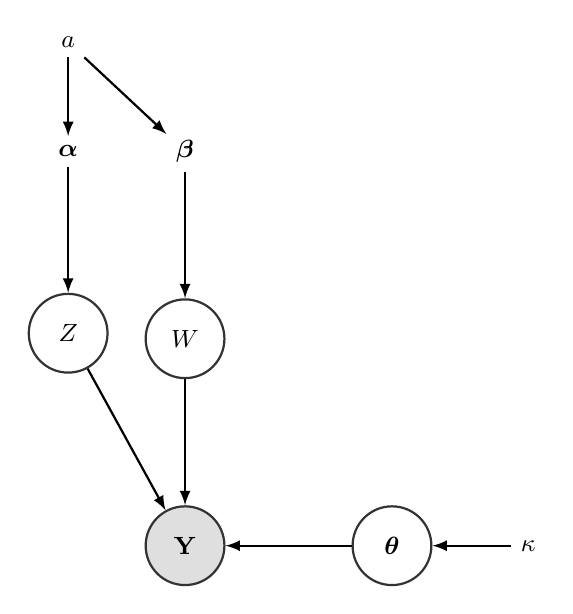
\begin{tikzpicture}
		\tikzstyle{main}=[circle, minimum size = 10mm, thick, draw =black!80, node distance = 16mm]
		\tikzstyle{connect}=[-latex, thick]
		%\tikzstyle{box}=[rectangle, draw=black!100]
		\node[ fill = white!100] (alpha) {$\boldsymbol{\alpha}$};
		\node[main] (Z) [below=of alpha] {$Z$};
		
		\node[] (a) [above= of alpha] {$a$}; 
		
		\node[] (beta) [right=of alpha] {$\boldsymbol{\beta}$};
		\node[main] (W) [below=of beta] {$W$};
		
		\node[main, fill = gray!25] (Y) [below=of W] {$\mathbf{Y}$};
		\node[main] (theta) [right=of Y] {$\boldsymbol{\theta}$};
		
		\node[] (kappa) [right=of theta] {$\kappa$};
		
		\path (Z) edge [connect] (Y);
		\path (W) edge [connect] (Y);
		
		\path (a) edge [connect] (alpha);
		\path (a) edge [connect] (beta);
		
		\path (theta) edge [connect] (Y);
		
		\path (alpha) edge [connect] (Z);
		\path (beta) edge [connect] (W);
		
		\path (kappa) edge [connect] (theta);

	\end{tikzpicture}
\end{figure}



\printbibliography

\end{document}